\documentclass[conference]{IEEEtran}
\IEEEoverridecommandlockouts
% The preceding line is only needed to identify funding in the first footnote. If that is unneeded, please comment it out.
\usepackage{cite}
\usepackage{amsmath,amssymb,amsfonts}
\usepackage{algorithmic}
\usepackage{graphicx}
\usepackage[brazilian]{babel}
\usepackage[utf8]{inputenc}
\usepackage[T1]{fontenc}
\usepackage{textcomp}
\usepackage{listings}
\usepackage{graphicx}

\def\BibTeX{{\rm B\kern-.05em{\sc i\kern-.025em b}\kern-.08em
    T\kern-.1667em\lower.7ex\hbox{E}\kern-.125emX}}
\begin{document}

\title{Simulação Biológica de Agrupamento de Formigas Mortas}

\author{\IEEEauthorblockN{1\textsuperscript{st} Marlon Henry Schweigert}
\IEEEauthorblockA{\textit{Departamento de Computação} \\
\textit{Centro de Ciências Tecnológicas - UDESC}\\
Joinville, Brasil \\
marlon.henry@magrathealabs.com}
\and
\IEEEauthorblockN{2\textsuperscript{nd} Rafael Stubs Parpinelli}
\IEEEauthorblockA{\textit{Departamento de Computação} \\
\textit{Centro de Ciências Tecnológicas - UDESC}\\
Joinville, Brasil \\
rafael.parpinelli@udesc.br}
}

\maketitle

\begin{abstract}
Este meta-artigo descreve o funcionamento computacional da simulação de formigas utilizando inteligência artificial dentro de um ambiente homogêneo visando simular o agrupamento de dados em lugares densos, realizando uma análise entre a variação dos parâmetros utilizados para o processamento da inteligência artificial.
\end{abstract}

\begin{IEEEkeywords}
formigas, inteligência artificial, modelagem matemática, programação concorrente
\end{IEEEkeywords}


\section{Introdução}

A busca por simular efeitos naturais que otimizem problemas em sistemas computacionais tem grandes vantagens comparados a algoritmos deterministas e objetivos, vistos que podemos dar sentido a resultados obtidos da natureza a qual algoritmos puramente matemáticos custam fazer qualquer sentido. Essa propriedade principal é aplicada ao algoritmo de aglomeração de formigas mortas por um grupo de formigas vivas.

O efeito de agrupamento de um ambiente poluído por formigas mortas foi descrito por XXX, a qual tem um sistema matemático pode descrever a movimentação de tais agentes.

\begin{figure}[h]
\centering
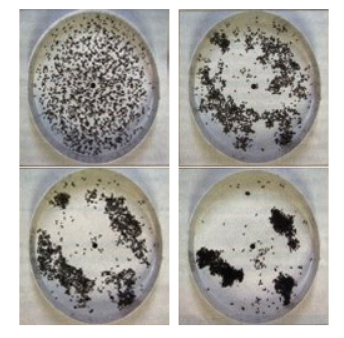
\includegraphics[width=2.5in]{clusters.png}
\caption{\textit{Clusters} de formigas mortas.}
\label{fig_sim}
\end{figure}

Tal comportamento é conhecido como agrupamento, na qual esse efeito pode ser utilizado para otimizar problemas de agrupamento, limpeza ou desfragmentação de ambientes na qual os dados manipulados sejam homogêneos.

Este artigo será dividido em algumas seções:

\begin{itemize}
    \item \textbf{Modelagem matemática}: Descreve as ações e o modelo matemático a qual os agentes podem realizar.
    \item \textbf{Resultados obtidos}: Amostras estado de execução obtidos da modelagem descrita, assim como métricas de recursos utilizados.
    \item \textbf{Análise sobre resultados obtidos}: Análise sobre estados obtidos e modelagem descrita.
\end{itemize}

\section{Modelagem matemática}

O ambiente onde ocorrerá a simulação é desenhado como uma matriz. A fim de descrever matematicamente o comportamento de agrupamento de formigas mortas em tal ambiente, precisamos tomar alguns conceitos de como o fenômeno ocorre:

\begin{itemize}
    \item Sem comunicação entre agentes: As formigas não utilizam nenhum método de comunicação entre outras formigas vivas para realizar este comportamento.
    \item Esse comportamento sempre é executado visando melhorar o caminho do ambiente.
    \item As ações tomadas podem ser descritas como:
    \begin{itemize}
        \item Pegar formiga;
        \item Soltar formiga;
        \item Caminhar;
    \end{itemize}
    \item As únicas percepções que a formiga utiliza para tomada de decisão são:
    \begin{itemize}
        \item Densidade da região onde ela está, utilizando um raio de visão.
        \item Se em sua atual posição existe ou não uma formiga.
    \end{itemize}
\end{itemize}

Dada essas características, podemos modelar as ações da formiga como uma cadeia de Markov a qual suas ações futuras requerem do seu estado atual. Essa cadeia de Markov é exibida na figura \ref{fig:automata}.

\begin{figure}[ht]
\centering
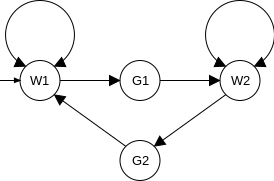
\includegraphics[width=2.5in]{how_walk_1.png}
\caption{Automato de estado de cada formiga.}
\label{fig:automata}
\end{figure}

Os estados descritos na figura \ref{fig:automata} são:

\begin{itemize}
    \item W1: Andando sem carregar uma formiga morta.
    \item G1: Pegar alguma formiga. Este estado tem uma probabilidade calculada dinamicamente conforme a posição atual da formiga.
    \item W2: Andando com uma formiga morta.
    \item G2: Soltar uma formiga morta. Este estado tem uma probabilidade calculada dinamicamente conforme o local da formiga.
\end{itemize}

Para este modelo funcionar, precisamos de um raio de visão ($R$), a qual significa quantas casas ao seu redor uma formiga pode observar. Esse parâmetro pode ser observado na figura \ref{fig:raio}.

\begin{figure}[h]
\centering
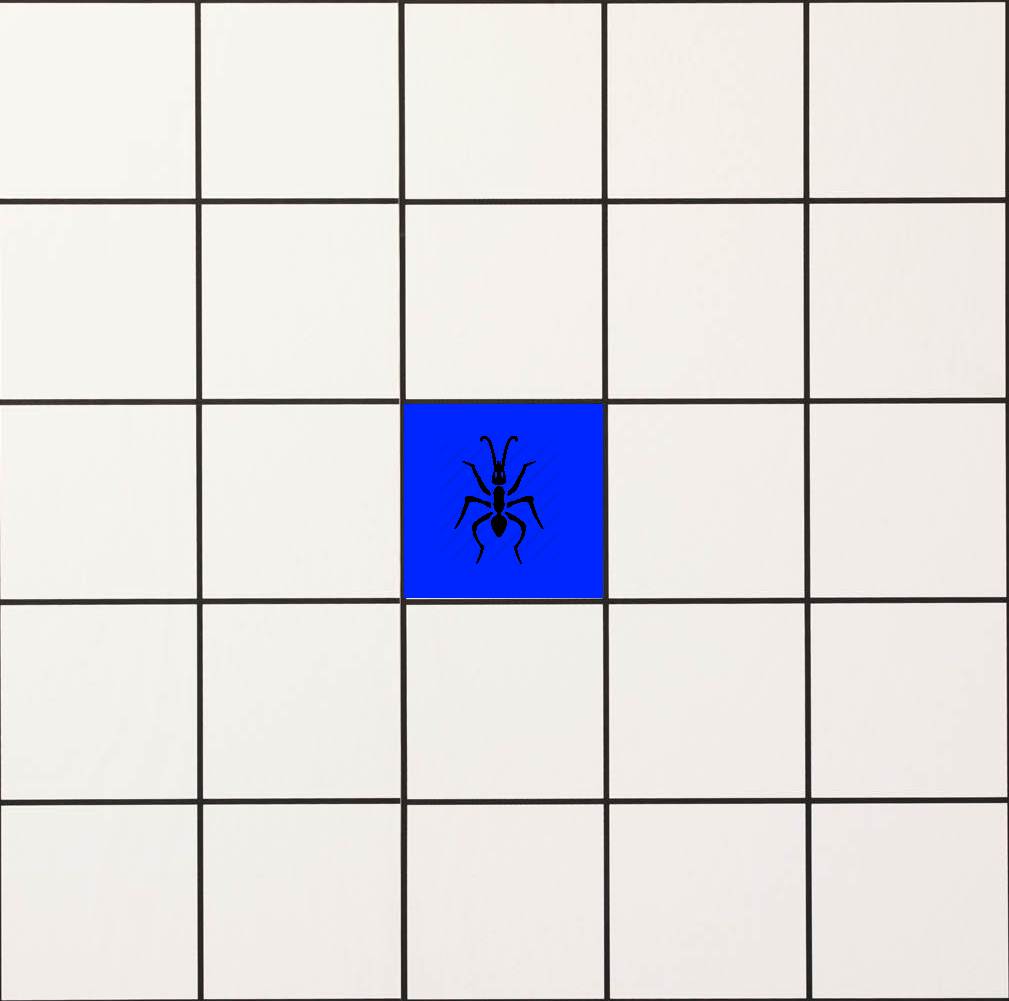
\includegraphics[width=2.5in]{formiga.png}
\caption{Formiga sobre a matriz, utilizando raio de visão 2.}
\label{fig:raio}
\end{figure}

O fator de decisão principal para pegar e soltar uma formiga morta está em torno da variável $D$ a qual é definida pela densidade local de cada formiga em torno do raio $R$ de cada formiga.


$D = \sum_{i=-R}^{R}\sum_{j=-R}^{R}A(i,j)$, onde

$A(i,j) =
\begin{array}{ll}
    1, if(has\_ant\_at(i,j))\\
    0
\end{array}
$

A abordagem desta simulação utiliza uma memória para cada formiga onde é armazenado qual a maior densidade ($D_{max}$) a qual esta formiga encontrou em sua vivência com o ambiente de testes. Essa informação é útil para normalizar dentro de um valor real [0, 1] a variável de Densidade relativa ($D_{rel}$). A fórmula de normalização é dada por:

$
    D_{rel} = \frac{D}{D_{max}}
$

Por fim, o modo de pensar da formiga é dado por tal algoritmo:

\lstinputlisting[language=Python]{ants.py}

Tal simulação foi criada em Golang para ter alto desempenho, facilidade de escritas de imagens e programação paralela facilitada.

Para funcionamento geral, executamos algumas threads onde cada thread manipula um conjunto de formigas. Cada formiga executará o algoritmo descrito acima por n vezes. Ao final, caso alguma formiga esteja carregando alguma formiga morta, elas executam paços até encontrarem um local bom para soltar e deixam de executar.

\section{Resultados Obtidos}

Utilizando $R=1$ foram obtidos as amostras (\ref{fig:r1}), a qual demonstram o agrupamento funcional mesmo pouca informação global para cada agente. Em comparativo a amostra obtida com $R=5$ (\ref{fig:r5}), as bordas são bem mais definidas no teste executado com $R=1$, porém em contra partida os grupos são mais definidos com $R=5$.

\begin{figure}[h!] 
  \begin{minipage}[b]{0.5\linewidth}
    \label{fig:r1} 
    \centering
    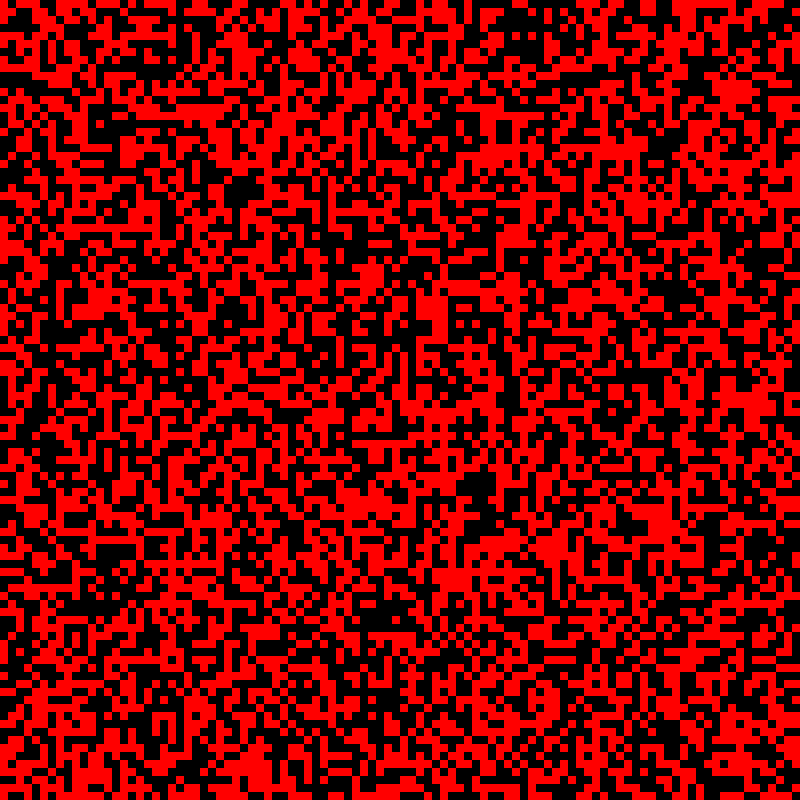
\includegraphics[width=.8\linewidth]{resultados/1-0.png} 
    \caption{Estado inicial com R=1} 
    \vspace{4ex}
  \end{minipage}%%
  \begin{minipage}[b]{0.5\linewidth}
    \centering
    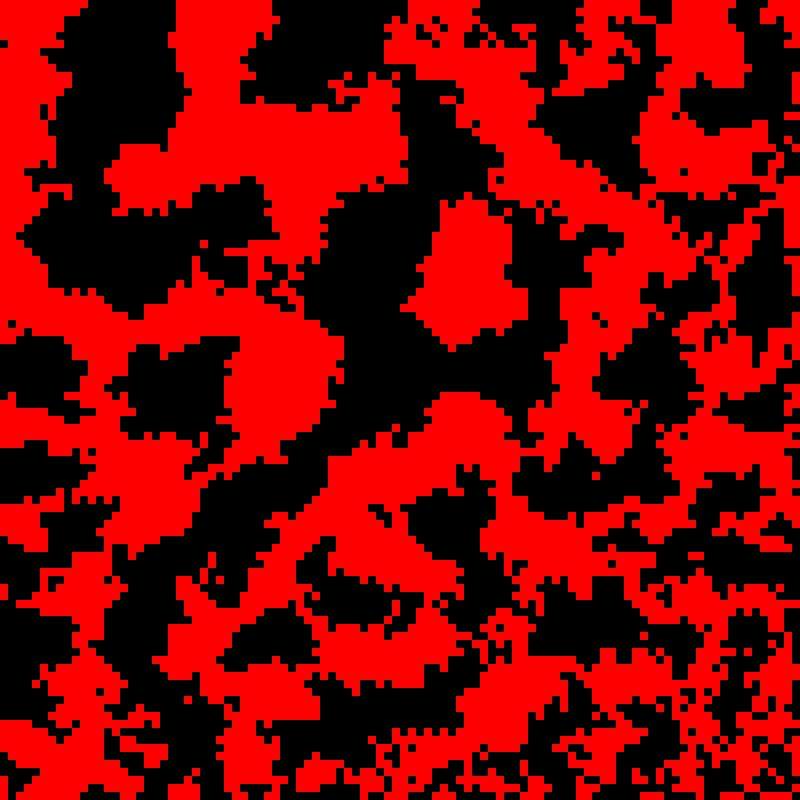
\includegraphics[width=.8\linewidth]{resultados/1-1.png} 
    \caption{100000 passos com R=1} 
    \vspace{4ex}
  \end{minipage} 
  \begin{minipage}[b]{0.5\linewidth}
    \centering
    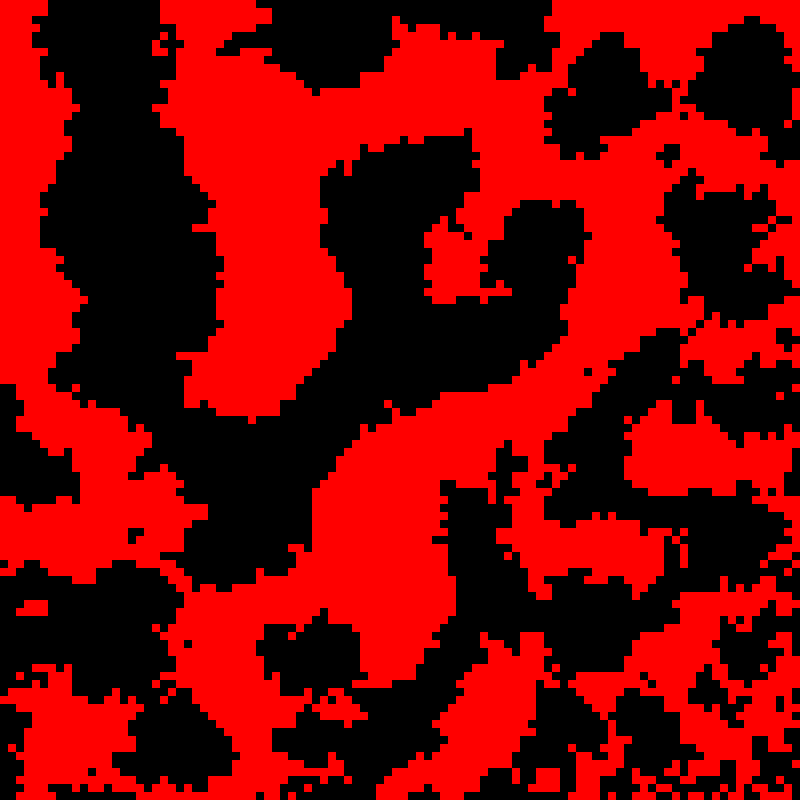
\includegraphics[width=.8\linewidth]{resultados/1-3.png} 
    \caption{300000 passos com R=1} 
    \vspace{4ex}
  \end{minipage}%% 
  \begin{minipage}[b]{0.5\linewidth}
    \centering
    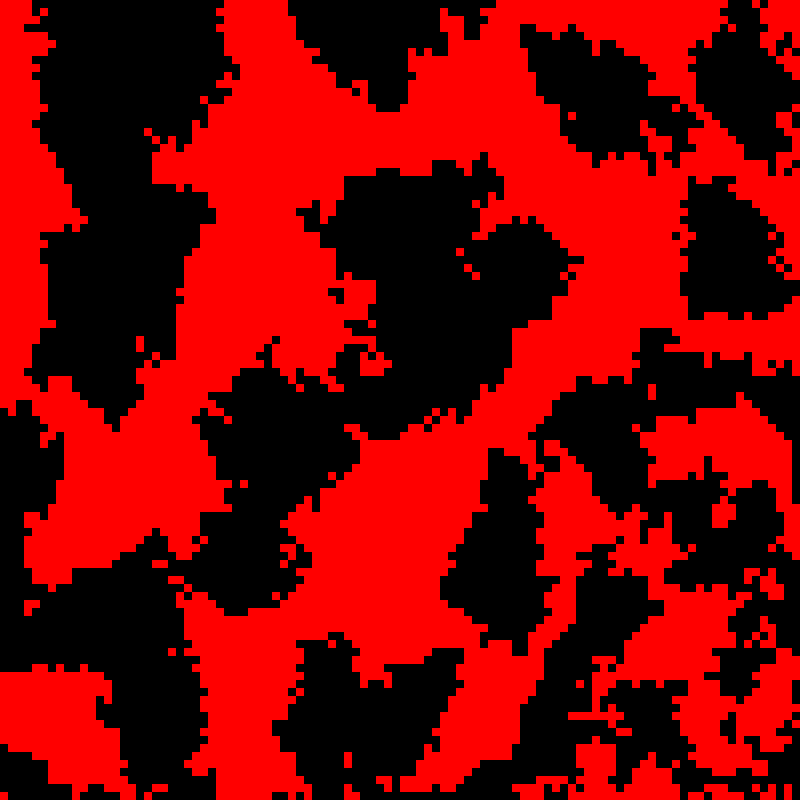
\includegraphics[width=.8\linewidth]{resultados/1-6.png} 
    \caption{500000 passos com R=1} 
    \vspace{4ex}
  \end{minipage} 
\end{figure}


\begin{figure}[h!]
  \begin{minipage}[b]{0.5\linewidth}
    \label{fig:r5} 
    \centering
    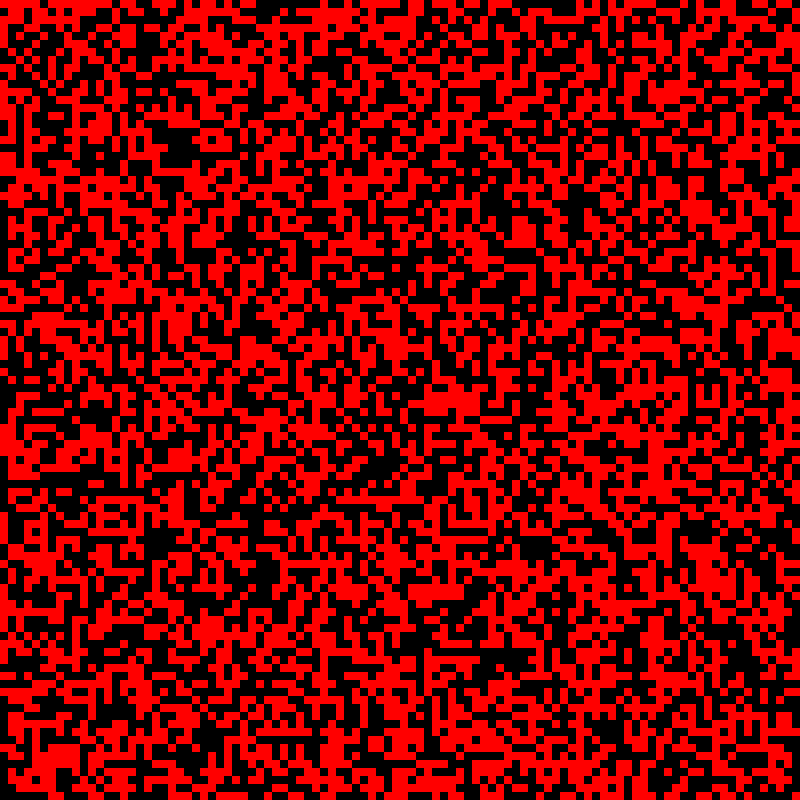
\includegraphics[width=.8\linewidth]{resultados/5-0.png} 
    \caption{Estado inicial com R=5} 
    \vspace{4ex}
  \end{minipage}%%
  \begin{minipage}[b]{0.5\linewidth}
    \centering
    
\includegraphics[width=.8\linewidth]{resultados/5-1.png} 
    \caption{100000 passos com R=5} 
    \vspace{4ex}
  \end{minipage} 
  \begin{minipage}[b]{0.5\linewidth}
    \centering
    
\includegraphics[width=.8\linewidth]{resultados/5-3.png} 
    \caption{300000 passos com R=5} 
    \vspace{4ex}
  \end{minipage}%% 
  \begin{minipage}[b]{0.5\linewidth}
    \centering
    
\includegraphics[width=.8\linewidth]{resultados/5-6.png} 
    \caption{500000 passos com R=5} 
    \vspace{4ex}
  \end{minipage} 
\end{figure}

Podemos ver um agravante na fragmentação das bordas dos grupos utilizando raio 10 (\ref{fig:r10}). Além disso, podemos perceber que o agrupamento nos primeiros passos, entre 0 e 100000 passos é muito mais custoso a ocorrer comparado aos raios menores.


\begin{figure}[h!] 
  \begin{minipage}[b]{0.5\linewidth}
    \label{fig:r10}
    \centering
    
\includegraphics[width=.8\linewidth]{resultados/10-0.png} 
    \caption{Estado inicial com R=10} 
    \vspace{4ex}
  \end{minipage}%%
  \begin{minipage}[b]{0.5\linewidth}
    \centering
    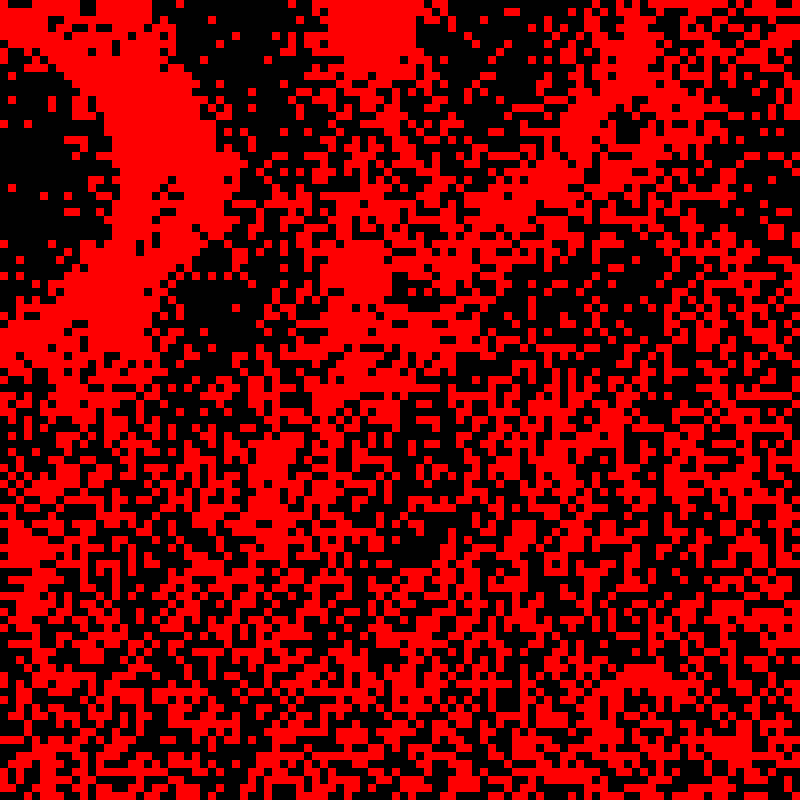
\includegraphics[width=.8\linewidth]{resultados/10-1.png} 
    \caption{100000 passos com R=10} 
    \vspace{4ex}
  \end{minipage} 
  \begin{minipage}[b]{0.5\linewidth}
    \centering
    
\includegraphics[width=.8\linewidth]{resultados/10-3.png} 
    \caption{300000 passos com R=10} 
    \vspace{4ex}
  \end{minipage}%% 
  \begin{minipage}[b]{0.5\linewidth}
    \centering
    
\includegraphics[width=.8\linewidth]{resultados/10-6.png} 
    \caption{500000 passos com R=10} 
    \vspace{4ex}
  \end{minipage} 
\end{figure}

Podemos assumir então, que quanto maior o raio, mais disperso será as bordas dos grupos. Isso é dado pela quebra de sistemas emergentes, visito que cada agente está levando em conta uma região muito grande ao invés de se preocupar com poucas informações.

\begin{thebibliography}{00}
\bibitem{b1} G. Eason, B. Noble, and I. N. Sneddon, ``On certain integrals of Lipschitz-Hankel type involving products of Bessel functions,'' Phil. Trans. Roy. Soc. London, vol. A247, pp. 529--551, April 1955.
\bibitem{b2} J. Clerk Maxwell, A Treatise on Electricity and Magnetism, 3rd ed., vol. 2. Oxford: Clarendon, 1892, pp.68--73.
\bibitem{b3} I. S. Jacobs and C. P. Bean, ``Fine particles, thin films and exchange anisotropy,'' in Magnetism, vol. III, G. T. Rado and H. Suhl, Eds. New York: Academic, 1963, pp. 271--350.
\bibitem{b4} K. Elissa, ``Title of paper if known,'' unpublished.
\bibitem{b5} R. Nicole, ``Title of paper with only first word capitalized,'' J. Name Stand. Abbrev., in press.
\bibitem{b6} Y. Yorozu, M. Hirano, K. Oka, and Y. Tagawa, ``Electron spectroscopy studies on magneto-optical media and plastic substrate interface,'' IEEE Transl. J. Magn. Japan, vol. 2, pp. 740--741, August 1987 [Digests 9th Annual Conf. Magnetics Japan, p. 301, 1982].
\bibitem{b7} M. Young, The Technical Writer's Handbook. Mill Valley, CA: University Science, 1989.
\end{thebibliography}

\end{document}
